
%Contribution of Authors and Co-Authors Page
%\title{CHAPTER X \\ MICROBURST SCALE SIZE DERIVED FROM MULTIPLE BOUNCES OF A MICROBURST SIMULTANEOUSLY OBSERVED WITH THE FIREBIRD-II CUBESATS}

\chapter{MICROBURST SCALE SIZE DERIVED FROM MULTIPLE BOUNCES OF A MICROBURST SIMULTANEOUSLY OBSERVED WITH THE FIREBIRD-II CUBESATS} \label{CH:bouncing_packet}

\section{Contribution of Authors and Co-Authors} 
\noindent Manuscript in Chapter 1 \\ 

\noindent Author: Mykhaylo Shumko 
\begin{singlespace} \noindent Contributions: Found bouncing packet microburst and analyzed its size and bounce period.  \end{singlespace}
\noindent Co-Author: John Sample  \\
\noindent Contributions: Provided advise and ideas. \\
\noindent Co-Author: Arlo Johnson \\
\noindent Contributions: Helped estimate the time corrections necessary for this analysis. \\
\noindent Co-Author: Bern Blake \\
\noindent Contributions: Provided advise and ideas. \\
\noindent Co-Author: Alex Crew\\
\noindent Contributions: Requested data and built the FIREBIRD-II CubeSats. \\
\noindent Co-Author: Harlan Spence\\
\noindent Contributions: FIREBIRD-II principal investigator. \\
\noindent Co-Author: Kavid Klumpar \\
\noindent Contributions: FIREBIRD-II principal investigator.  \\
\noindent Co-Author: Oleksiy Agapitov \\
\noindent Contributions: Provided guidance to calculate the microburst bounce period. \\
\noindent Co-Author: Matthew Handley \\
\noindent Contributions: Downloaded data and built the FIREBIRD-II CubeSats.

\newpage


\section{Manuscript Information}

\begin{singlespace} \noindent Mykhaylo Shumko, John Sample, Arlo Johnson, Bern Blake, Alex Crew, Harlan Spence, David Klumpar, Oleksiy Agapitov, and Matthew Handley \end{singlespace}

\begin{singlespace}
\noindent Status of Manuscript: \\
\_\_\_ Prepared for submission to a peer-reviewed journal \\
\_\_\_ Officially submitted to a peer-reviewed journal \\
\_\_\_ Accepted by a peer-reviewed journal \\ 
\_X\_ Published in a peer-reviewed journal
\end{singlespace}

\begin{singlespace}
\noindent Geophysical Research Letters Volume 45, Issue 17 \\
\noindent DOI: 10.1029/2018GL078925
\end{singlespace} 

\noindent This article is available under the terms of the Creative Commons Attribution Non-Commercial No Derivatives License CC BY-NC-ND (which may be updated from time to time) and permits non-commercial use, distribution, and reproduction in any medium, without alteration, provided the original work is properly cited and it is reproduced verbatim.

\newpage

\section{Key Points}
\begin{itemize}
\item Multiple bounces from a microburst were observed by the two FIREBIRD-II CubeSats at LEO.
\item The lower bounds on the microburst scale size at LEO were $29 \pm 1$ km (latitudinal) and $51 \pm 11$ km (longitudinal).
\item Deduced lower bound equatorial scale size was similar to the whistler-mode chorus source scale.
\end{itemize}

%% ------------------------------------------------------------------------ %%
%
%  ABSTRACT
%
% A good abstract will begin with a short description of the problem
% being addressed, briefly describe the new data or analyses, then
% briefly states the main conclusion(s) and how they are supported and
% uncertainties. 
%% ------------------------------------------------------------------------ %%

%% \begin{abstract} starts the second page 

\section{Abstract}
We present the observation of a spatially large microburst with multiple bounces made simultaneously by the FIREBIRD-II CubeSats on February 2nd, 2015. This is the first observation of a microburst with a subsequent decay made by two co-orbiting but spatially separated spacecraft. From these unique measurements, we place estimates on the lower bounds of the spatial scales as well as quantify the electron bounce periods. The microburst's lower bound latitudinal scale size was $29 \pm 1$ km and the longitudinal scale size was $51 \pm 1$  km in low earth orbit. We mapped these scale sizes to the magnetic equator and found that the radial and azimuthal scale sizes were at least $500 \pm​ 10$ km and $530 \pm 10$ km, respectively. These lower bound equatorial scale sizes are similar to whistler-mode chorus wave source scale sizes, which supports the hypothesis that microbursts are a product of electron scattering by chorus waves. Lastly, we estimated the bounce periods for 200-800 keV electrons and found good agreement with four common magnetic field models.

%% ------------------------------------------------------------------------ %%
%
%  TEXT
%
%% ------------------------------------------------------------------------ %%
\section{Introduction}\label{Intro}
The dynamics of radiation belt electrons are complex, and are driven by competition between source and loss processes. A few possible loss processes are radial diffusion \citep{Shprits2004}, magnetopause shadowing \citep{Ukhorskiy2006}, and pitch angle and energy diffusion due to scattering of electrons by plasma waves \citep[e.g.][]{Abel1998_1, Summers1998, Meredith2002, Selesnick2003, Horne2003, Thorne2005, Mozer2018}. There are a variety of waves that cause pitch angle scattering, including electromagnetic ion cyclotron waves, plasmaspheric hiss, and chorus \citep{Millan2007, Thorne2010}. Chorus predominantly occurs in the dawn sector (6-12 magnetic local times (MLT)) \citep{Li2009} where it accelerates electrons with large equatorial pitch angles and scatters electrons with small equatorial pitch angles \citep{Horne2003}. Some of these electrons may be impulsively scattered into the loss cone, where they result in short-duration ($\sim 100$ ms) enhancements in precipitating flux called microbursts.

\citet{Anderson1964} coined the term microburst to describe high altitude balloon observations of $\sim 100$ ms duration enhancements of bremsstrahlung X-rays emitted from scattered microburst electrons impacting the atmosphere. Since then, non-relativistic (less than a few hundred keV) microbursts have been routinely observed with other balloon missions \citep[e.g.][]{Parks1967, Woodger2015, Anderson2017}. A review of the literature shows no reports of microbursts above a few hundred keV observed by balloons \citep{Millan2002, Woodger2015}. This lack of observation may be explained by relatively weaker pitch angle scattering of relativistic electrons by chorus \citep{Lee2012}. 

In addition to the X-ray signature for bursts of electron precipitation, the precipitating relativistic and non-relativistic electrons have been measured in situ by spacecraft orbiting in low earth orbit (LEO). Hereinafter, we refer to these electron signatures observed by LEO spacecraft also as microbursts. Microbursts have been observed with, e.g. the Solar Anomalous and Magnetospheric Particle Explorer's (SAMPEX) > 150 keV and > 1 MeV channels \citep{Nakamura1995, Nakamura2000, Blake1996, Lorentzen2001a, Lorentzen2001b, O'Brien2003, O'Brien2004, Blum2015} and Focused Investigation of Relativistic Electron Bursts: Intensity, Range, and Dynamics (FIREBIRD-II) with its > 200 keV energy channels \citep{Crew2016, Anderson2017, Breneman2017}.

Understanding microburst precipitation and its scattering mechanism is important to radiation belt dynamics. The scattering mechanism has been observationally studied by e.g. \citet{Lorentzen2001b} who found that microbursts and chorus waves predominantly occur in the dawn sector and \citet{Breneman2017} made a direct observational link between individual microbursts and chorus elements. Microbursts have been modeled and empirically estimated to be capable of depleting the relativistic electron population in the outer radiation belt on the order of a day \citep{O'Brien2004, Thorne2005, Shprits2007, Breneman2017}. An important parameter in this estimation of instantaneous radiation belt electron losses due to microbursts is their scale size. \citet{Parks1967} used balloon measurements of bremsstrahlung X-rays to estimate the high altitude scale size of predominantly low energy microbursts to be $40 \pm 14$ km. In \citet{Blake1996} a microburst with multiple bounces was observed by SAMPEX, and the microburst's latitudinal scale size in LEO was estimated to have been ``at least a few tens of kilometers". \citet{Blake1996} concluded that typically microbursts are less than a few tens of electron gyroradii in size (at L = 5 at LEO, the gyroradii of 1 MeV electrons is on the order of 100 m). \citet{Dietrich2010} used SAMPEX along with ground-based very low frequency stations to conclude that during one SAMPEX pass, the observed microbursts had scale sizes less than $4$ km.

Since February 1st, 2015, microbursts have been observed by FIREBIRD-II, a pair of CubeSats in LEO. Soon after launch, when the two FIREBIRD-II spacecraft were at close range, a microburst with a scale size greater than 11 km was observed \citep{Crew2016}. On the same day, FIREBIRD-II simultaneously observed a microburst with multiple bounces. The microburst decay was observed over a period of a few seconds, while the spacecraft were traveling predominantly in latitude. Here we present the analysis and results of the latitude and longitude scale sizes and bounce periods of the first microburst with multiple bounces observed with the two FIREBIRD-II spacecraft.

\section{Spacecraft and Observation} \label{obs} %%%%%%%%%%%%%%%%%%%%%%%%%%%%%%%%%%%%%%%%%%%%%%%%%%%%%%%%%%%%%%%%%%%%%%%%%%
The FIREBIRD missions are comprised of a pair of identically-instrumented 1.5U CubeSats (15 x 10 x 10 cm) that are designed to measure electron precipitation in LEO \citep{Spence2012, Klumpar2015}. The second mission, termed FIREBIRD-II, was launched on January 31st 2015.  The two FIREBIRD-II CubeSats, identified as Flight Unit 3 (FU3) and Flight Unit 4 (FU4), were placed in a 632 km apogee, 433 km perigee, and $99^{\circ}$ inclination orbit \citep{Crew2016}. FU3 and FU4 are orbiting in a string of pearls configuration with FU4 ahead, to resolve the space-time ambiguity of microbursts. Each FIREBIRD-II unit has two solid state detectors: one is mounted essentially at the spacecraft surface, covered only by a thin foil acting as a sun shade, with a field of view of $90^{\circ}$ (surface detector), and the other is beneath a collimator which restricts the field of view to $54^{\circ}$ (collimated detector). Only FU3 has a functioning surface detector, so this analysis utilizes the collimated detectors. FU3's surface and collimated detectors, as well as FU4's collimated detector observe electron fluxes in six energy channels from $\sim 230$ keV to $> 1$ MeV. FIREBIRD-II's High Resolution (HiRes) electron flux data is gathered with an adjustable sampling period of 18.75 ms by default and can be as fast as 12.5 ms. 

On February 2nd, 2015 at 06:12 UT, both FIREBIRD-II spacecraft simultaneously observed an initial microburst, followed by subsequent periodic electron enhancements of diminishing amplitude shown in Fig. \ref{hires_plot}. This is thought to be the signature of a single burst of electrons, some of which precipitate, but the rest mirror near the spacecraft then bounce to the conjugate hemisphere where they mirror again and the subsequent bounces produce a train of decaying peaks \citep{Blake1996, Thorne2005}. This bounce signature occurred during the transition between the main and recovery phases of a storm with a minimum Dst of -44 nT (Kp = 4, and AE ${\approx 400}$ nT). At this time, the HiRes data was sampled at 18.75 ms. Five peaks were observed by both spacecraft. The fifth peak observed by FU4 was comparable to the Poisson noise and was not used in this analysis. This microburst was observed from the first energy channel ($\approx 200-300$ keV), to the fourth energy channel ($\approx 500-700$ keV), and FU3's surface detector observed the microburst up to the fifth energy channel (683 - 950 keV).

\begin{figure}
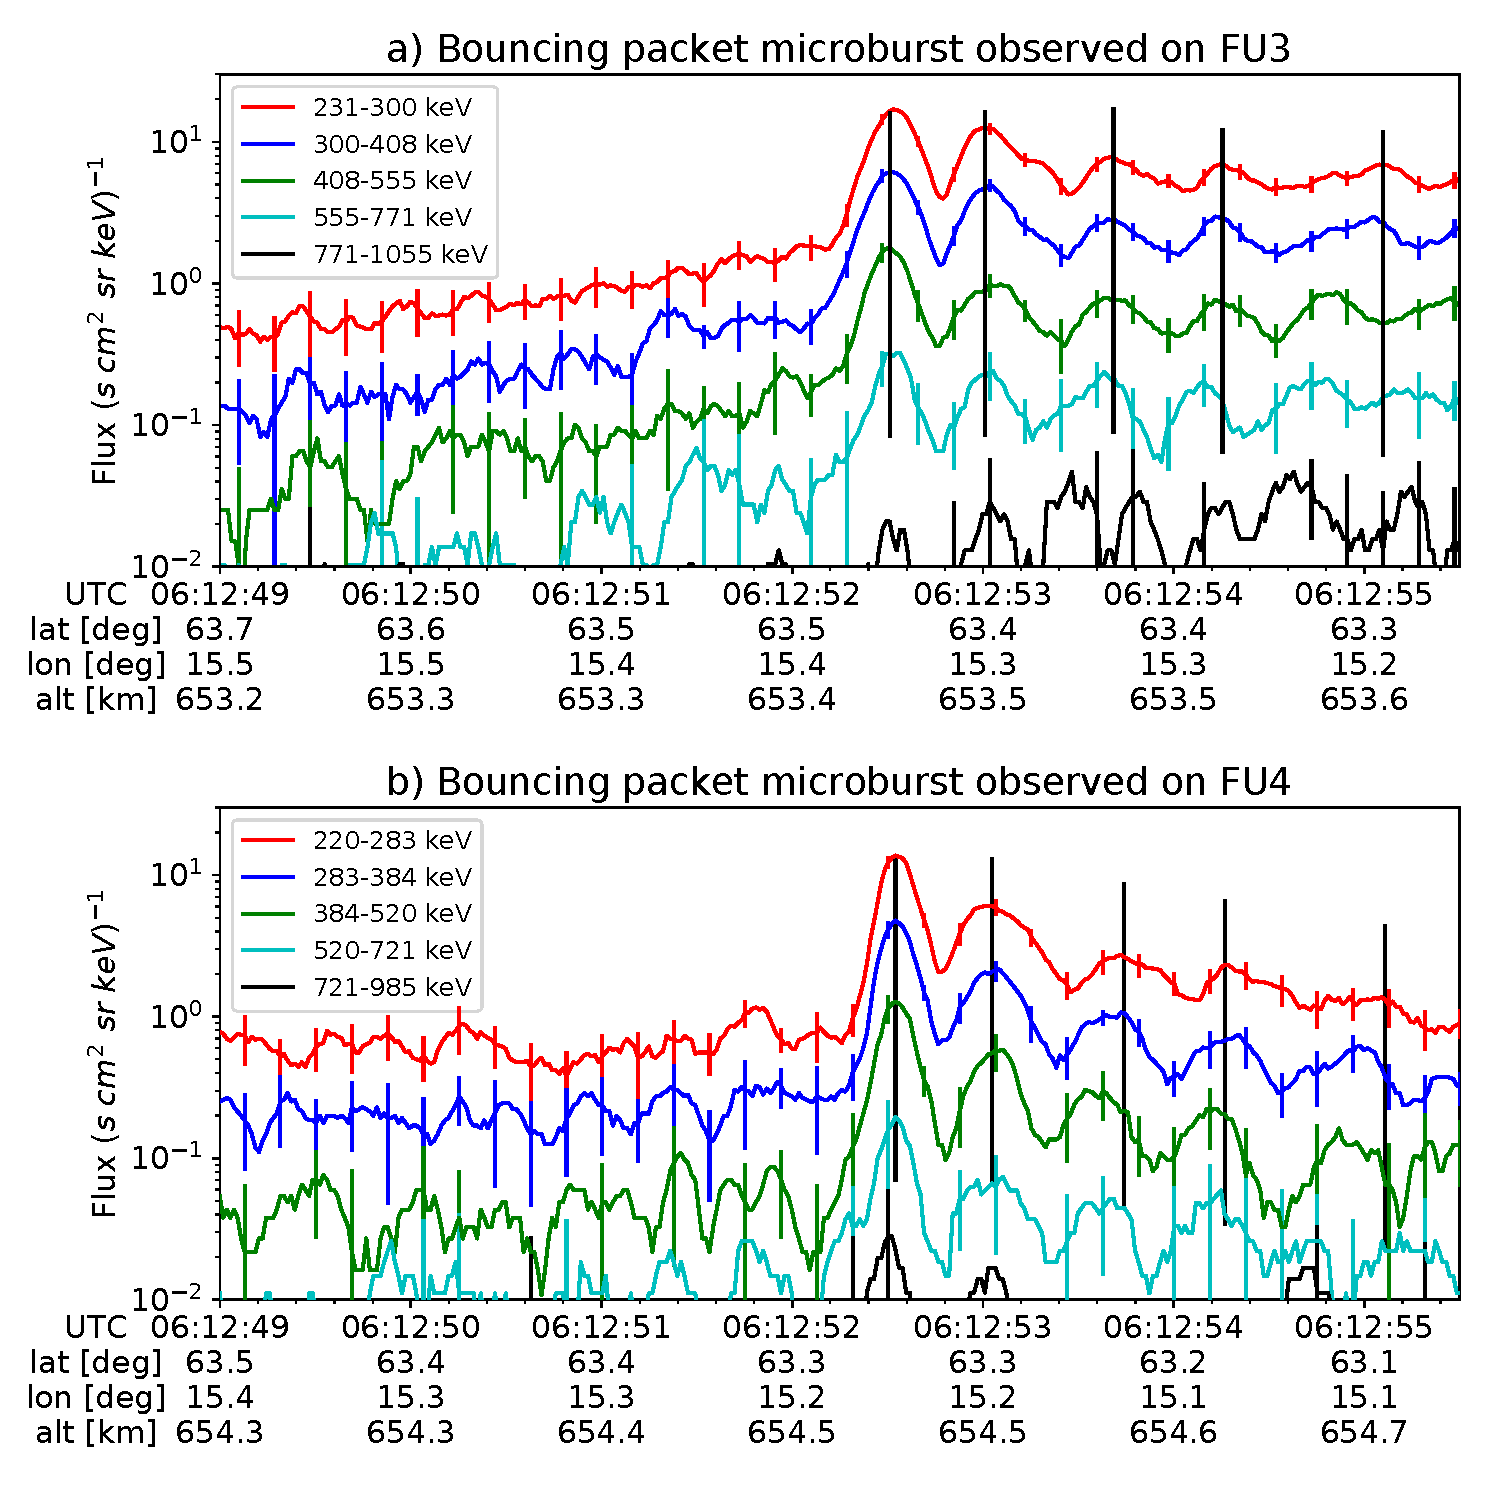
\includegraphics[width=\textwidth]{3_hires_plot_log_8pt_smooth_pos_v2.pdf}
\caption{HiRes data of the microburst observed at February 2nd, 2015 at 06:12:53 UT, smoothed with a 150 ms rolling average. The subsequent bounces showed some energy dispersion. As discussed in Appendix \ref{appendixb}, a time correction of -2.28 s was applied to FU3. While the flux from five energy channels is shown, only channels with reasonable counting statistics were used for the spatial scale analysis. Vertical colored bars show the $\sqrt{N}$ error every 10th data point and vertical black bars are lined up with the peaks in the 220-283 keV energy channel to help identify dispersion.}
\label{hires_plot}
\end{figure} 

The HiRes data in Fig. \ref{hires_plot} shows signs of energy dispersion, characterized by higher energy electrons arriving earlier than the lower energies. This time of flight energy dispersion tends to smear out the initial sharp burst upon each subsequent bounce. The first peak does not appear to be dispersed, and subsequent peaks show a dispersion trend consistent across energy channels. The black vertical bars have been added to Fig. \ref{hires_plot} to highlight this energy dispersion. This dispersion signature and amplitude decay implies that the first peak was observed soon after the electrons were scattered, followed by decaying bounces.

At this time, in magnetic coordinates, FIREBIRD-II was at McIlwain L = 4.7 and MLT = 8.3, calculated with the Tsyganenko 1989 (T89) magnetic field model \citep{Tsyganenko1989} using IRBEM-Lib \citep{irbem}. Geographically, they were above Sweden, latitude = $63^{\circ}$N, longitude = $15^{\circ}$E, altitude = 650 km. This geographic location is magnetically conjugate to the east of the so-called South Atlantic Anomaly (SAA). The SAA is the location where the mirror points of electrons tend to occur at locations deeper in the atmosphere owing to the offset of the dipole magnetic field from the Earth's center. Electrons with pitch angles within the drift loss cone (DLC) will encounter the SAA and be removed from their eastward longitudinal drift paths \citep{Comess2013, Dietrich2010}. FU3 and FU4 are therefore both in regions where the particles in the DLC have recently precipitated, leaving only particles that were recently scattered. At the spacecraft location, locally mirroring electrons would have mirrored at 95 km in the opposite hemisphere, with more field aligned electrons mirroring at even lower altitudes. From the analysis done by \citet{Fang2010}, the peak in the total ionization rate in the atmosphere for 100 keV electrons is around 80 km altitude, while the total ionization rate from 1 MeV electrons peaks around 60 km altitude. It is, therefore, expected that a fraction of the microburst electrons will survive each encounter with the atmosphere. By plotting the peak flux as a function of bounce (not shown), it was found that 40 - 60 \% of the microburst electrons were lost on the first bounce, similar to the 33\% loss per bounce observed for a bouncing microburst observed by SAMPEX \citep{Thorne2005}.

\section{Analysis} \label{analysis} %%%%%%%%%%%%%%%%%%%%%%%%%%%%%%%%%%%%%%%%%%%%%%%%%%%%%%%%%%%%%%%%%%%%%%%%%%%%%%%%%%%%%%%%%
At the beginning of the FIREBIRD-II mission, two issues prevented the proper analysis of the microburst's spatial scale size: the spacecraft clocks were not synchronized, and their relative positions were not accurately known. We addressed these issues with a cross-correlation time lag analysis described in detail in Appendix \ref{appendixb}. From this analysis, the time correction was $2.28 \pm 0.12$ s (applied to Fig. \ref{hires_plot}) and the separation was $19.9 \pm 0.9$ km at the time of the microburst observation.

\subsection{Electron Bounce Period} \label{t_b} %%%%%%%%%%%%%%%%%%%%%%%%%%%%%%%%%%%%%%%%%%%%%%%%%%%%%%%%%%%%%%%
We used this unique observation of bouncing electrons to calculate the bounce period, $t_b$ as a function of energy and compare it to the energy-dependent $t_b$ curves derived from four magnetic field models, the results of which are shown in Fig. \ref{tb_plot}. The observed $t_b$ and uncertainties were calculated by fitting the baseline-subtracted HiRes flux. The baseline flux used in this analysis is given in \citet{O'Brien2004} as the flux at the 10th percentile over a specified time interval, which in this analysis was taken to be 0.5 seconds. The flux was fitted with a superposition of Gaussians for each energy channel, and the uncertainty in flux was calculated using the Poisson error from the microburst and baseline fluxes summed in quadrature. Using the fit parameters, the mean $t_b$ for the lowest four energy channels is shown in Fig. \ref{tb_plot}. The trend of decreasing $t_b$ as a function of energy is evident in Fig. \ref{tb_plot}, which further supports the assumption that the subsequent peaks are bounces, and not a train of microbursts scattered by bouncing chorus. 

\begin{figure}
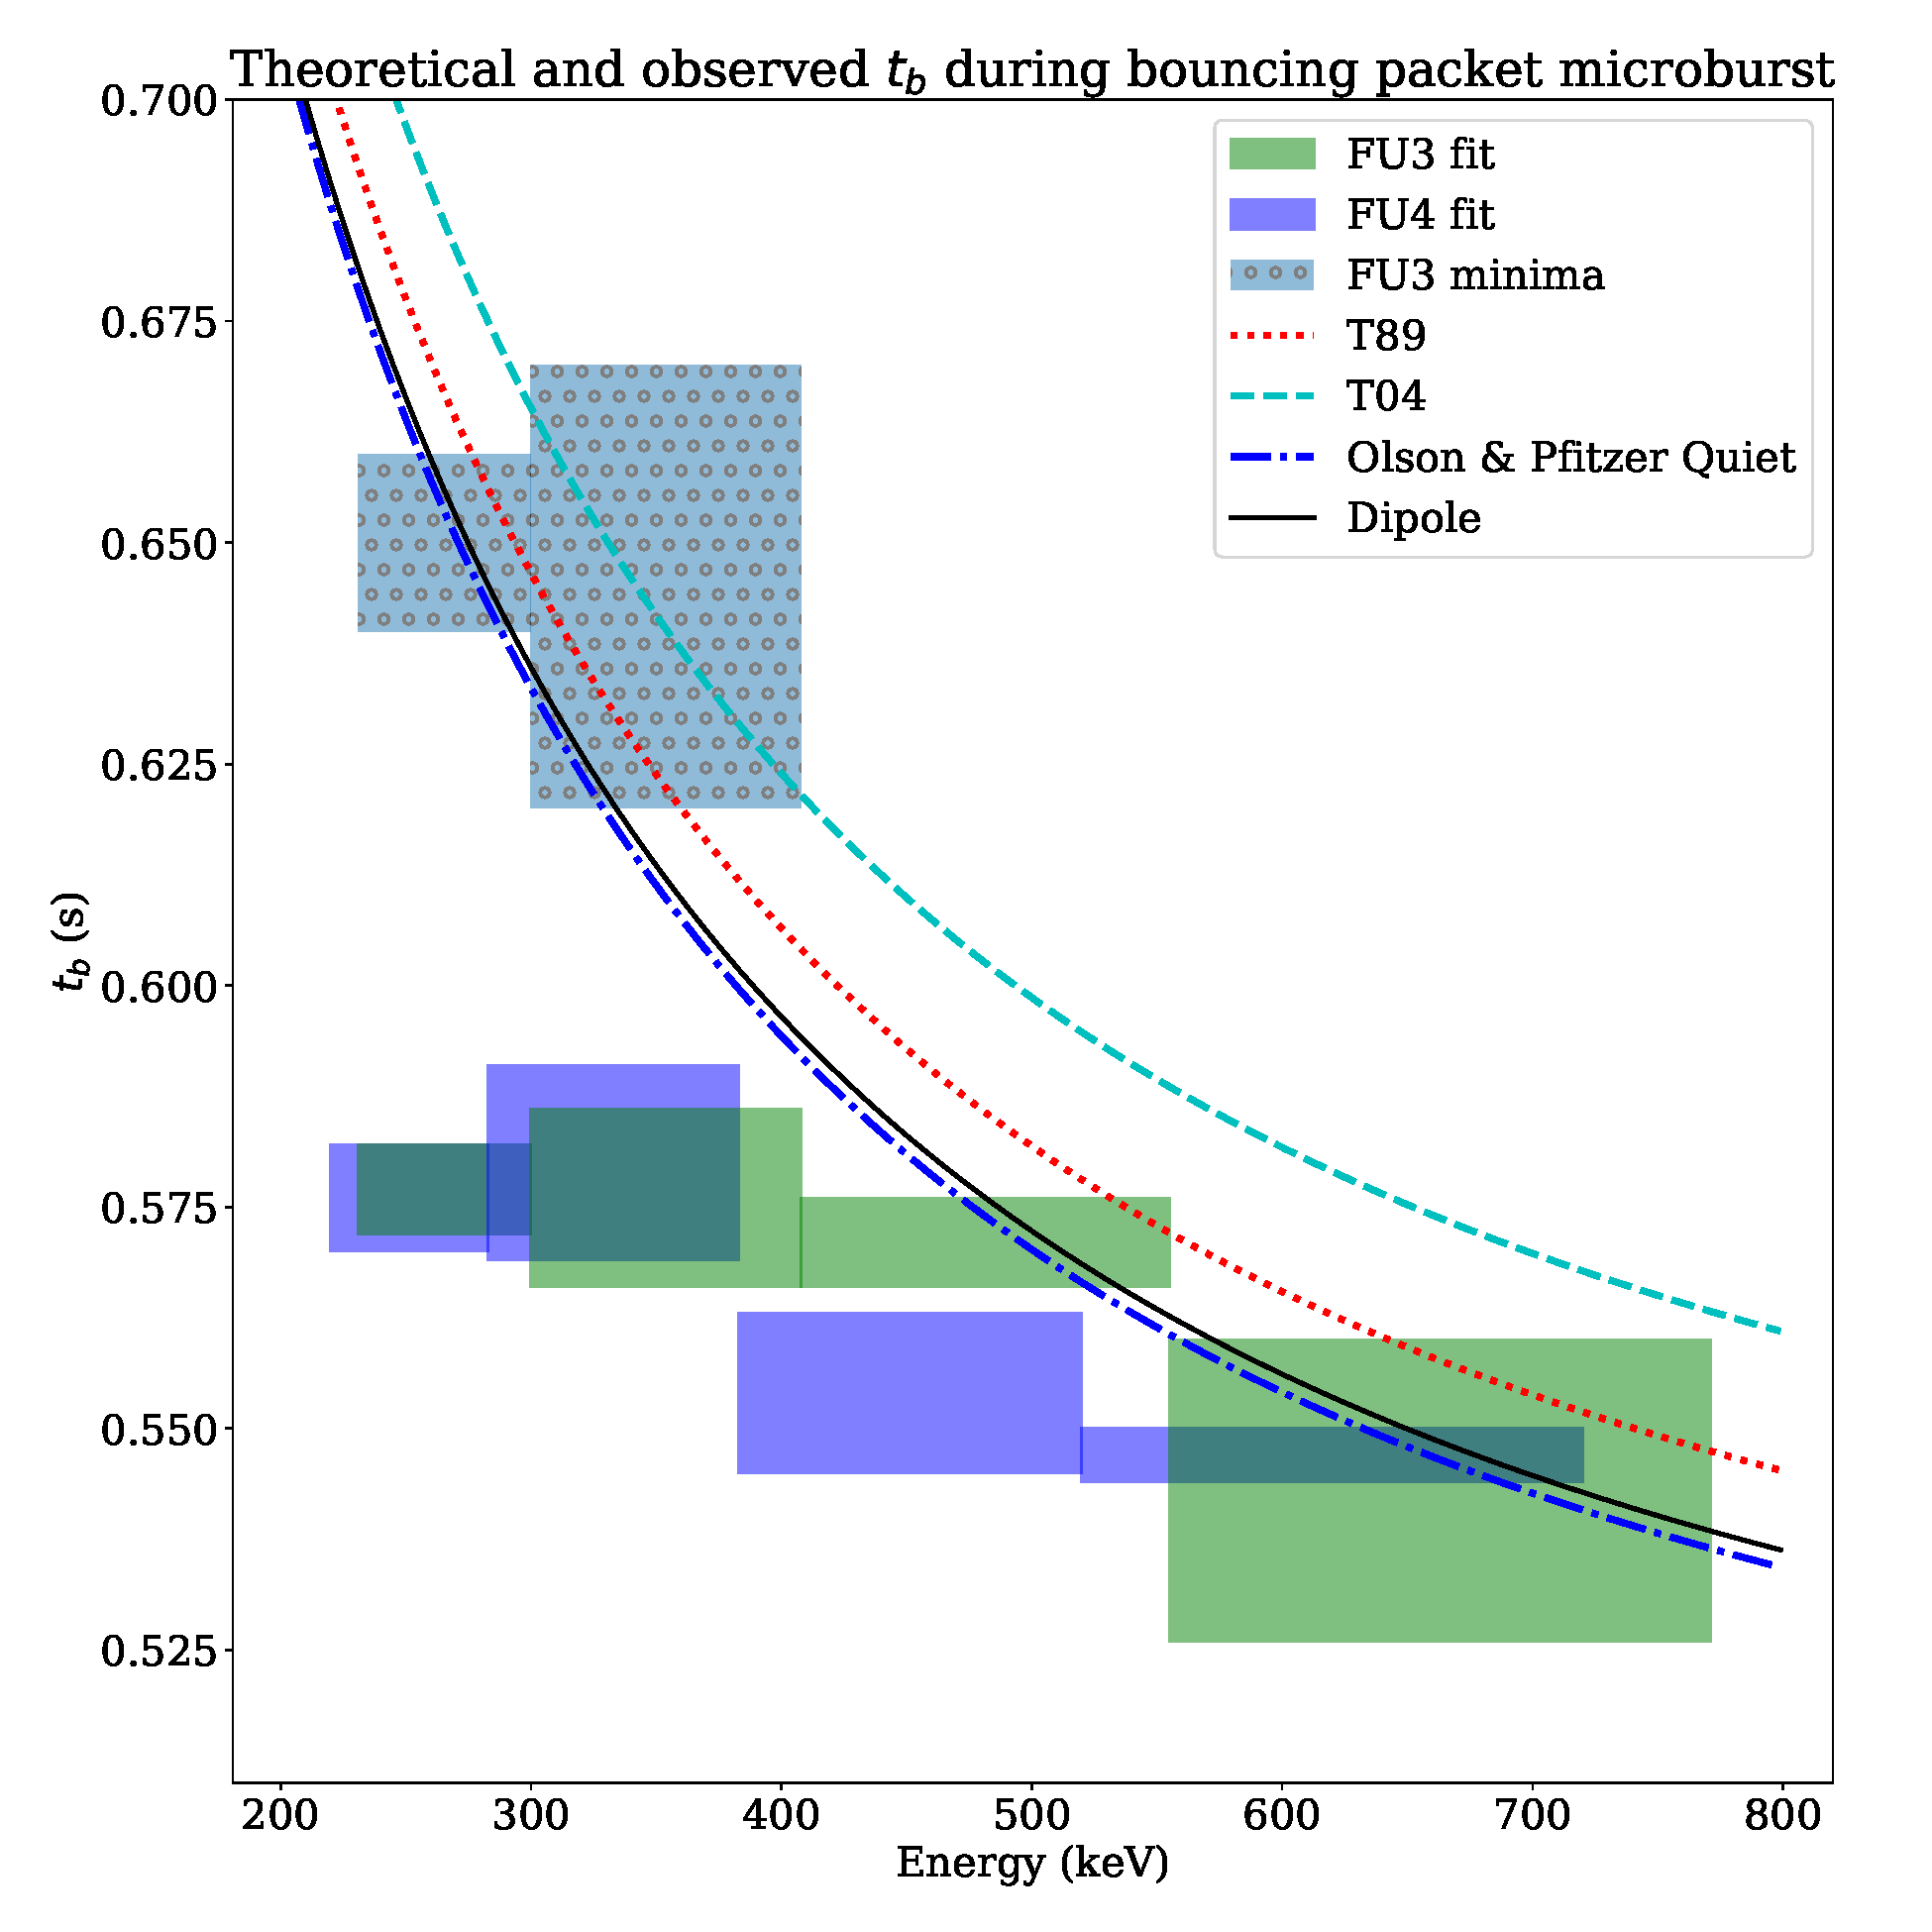
\includegraphics[width=\textwidth]{3_detrended_bounce_period_boxed_adj.pdf}
\caption{Observed and theoretical $t_b$ for electrons of energies from 200 to 770 keV. The solid black line is $t_b$ in a dipole magnetic field, derived in \citet{Schulz1974}. The red dotted and cyan dashed lines are the $t_b$ derived using the T89, and T04 magnetic field models with IRBEM-Lib. Lastly, the blue dot-dash curve is the $t_b$ derived using the Olson \& Pfitzer Quiet model. The green and purple rectangles represent the observed $t_b$ for FU3 and FU4 using a Gaussian fit, respectively. The blue rectangles represent the observed $t_b$ calculated with the minima between the bounces. The width of the boxes represent the width of those energy channels, and the height represents the uncertainty from the fit.}
\label{tb_plot}
\end{figure}

The decaying peaks in the 231-408 keV electron flux observed by FU3's lowest two energy channels (see Fig. \ref{hires_plot}) were right-skewed. One explanation is that there was in-channel energy dispersion within those channels. Since $t_b$ of higher energy electrons is shorter, a right-skewed peak implies that higher energy electrons were more abundant within that channel e.g. in FU3's 231-300 keV channel, the 300 keV electrons will arrive sooner than the 231 keV electrons, but will they will be binned in the same channel. A Gaussian fit cannot account for this in-channel dispersion, and as a first order correction, minima between peaks was used to calculate $t_b$, and is shown in Fig. \ref{tb_plot}. The observed energy-dependent dispersion shown in Fig. \ref{tb_plot} is consistent with higher energy peaks returning sooner. This dispersion consistency further supports the assumption that the subsequent peaks are bounces, and not a train of microbursts scattered by bouncing chorus.

To compare the observed and modeled $t_b$, we superposed $t_b$ curves for various models including an analytical solution in a dipole \citep{Schulz1974}, and numerical models: T89, Tsyganenko 2004 (T04) \citep{Tsyganenko2005}, and Olson \& Pfitzer Quiet \citep{Olson1982} in Fig. \ref{tb_plot}. The numerical $t_b$ curves were calculated using a wrapper for IRBEM-Lib. This code traces the magnetic field line between mirror points, and calculates $t_b$ assuming conservation of energy and the first adiabatic invariant for electrons mirroring at FIREBIRD-II. With the empirical $t_b$, the models agree within FIREBIRD-II's uncertainties, but the T04 model has the largest discrepancy compared to the other models.

\subsection{Microburst Energy Spectra}
Next, we investigated the energy spectra of this microburst. The energy spectra was modeled with an exponential that was fit to the peak flux derived from the Gaussian fit parameters in section \ref{t_b} to all but the highest energy channel. We found that the E-folding energy, $E_0 \sim 100$ keV. This spectra is similar to spectra show by \citet{Lee2005} from STSAT-1 and \citet{Datta1997} from sounding rocket measurements. The energy spectra is soft for a typical microburst observed with FIREBIRD-II and there was no statistically significant change in $E_0$ for subsequent bounces.

\subsection{Microburst Scale Sizes} \label{scale_size} %%%%%%%%%%%%%%%%%%%%%%%%%%%%%%%%%%%%%%%%%%%%%
Lastly, after we applied the time and separation corrections detailed in Appendix \ref{appendixb}, we mapped the locations of FU3 and FU4 in Fig. \ref{map_plot}. The locations where FU3 saw peaks 1-5 and where FU4 saw peaks 1-4 are shown as P1-5 and P1-4, respectively. The lower bound on the latitudinal extent of the microburst was the difference in latitude between P1 on FU3 and P4 on FU4 and was found to be $29 \pm 1$ km. The uncertainty was estimated from the spacecraft separation uncertainty described in Appendix \ref{appendixb}. This scale size is the largest reported by FIREBIRD-II.

\begin{figure}
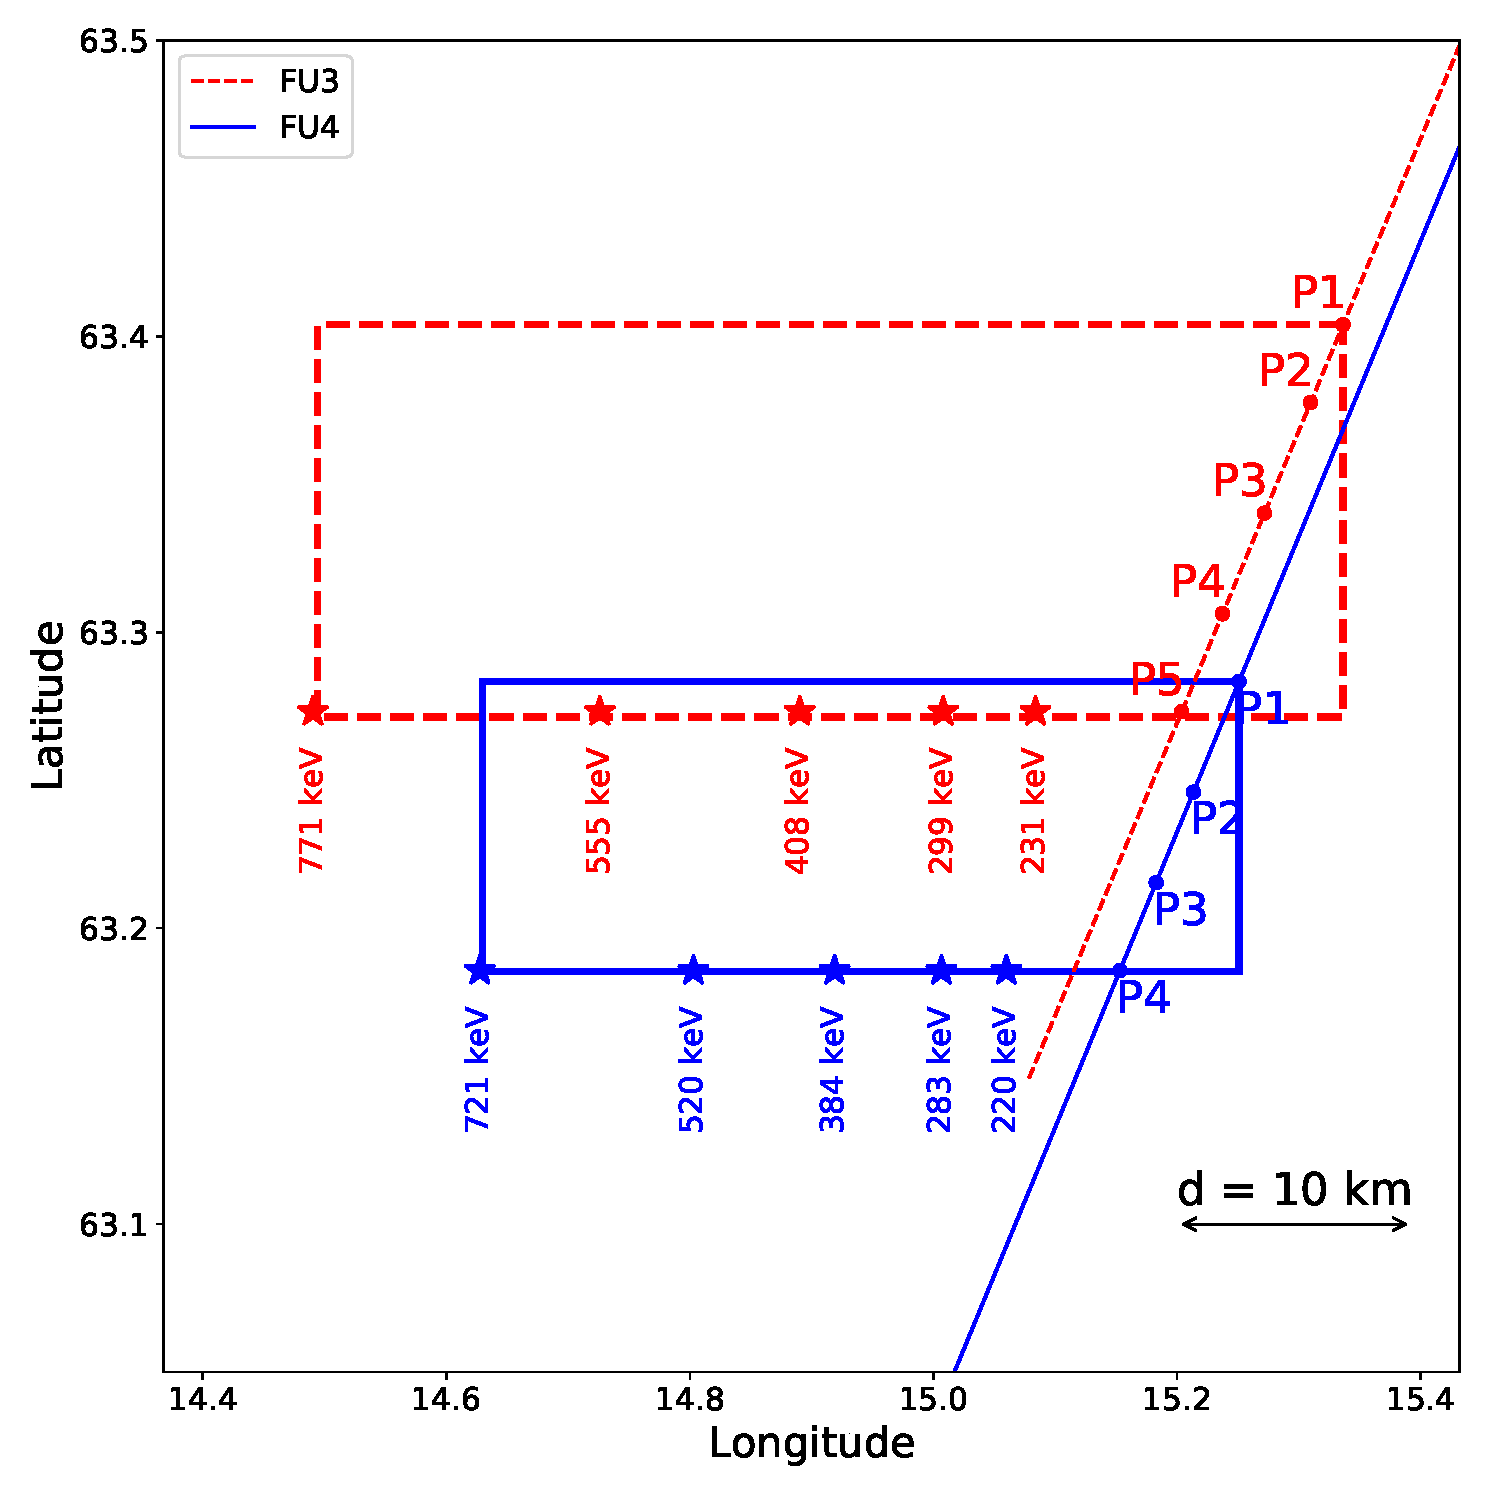
\includegraphics[width=\textwidth]{3_decay_microburst_distance_corrected_CH4_last_pk_drift_color_3.pdf}
\caption{The topology of the FIREBIRD-II orbit and the multiple bounces of the microburst projected onto latitude and longitude with axis scaled to equal distance. Attributes relating to FU3 shown in red dashed lines, and FU4 with blue solid lines. The spacecraft path is shown with the diagonal lines, starting at the upper right corner. The labels P1-4 for FU4 and P1-5 for FU3 indicate where the spacecraft were when the N$^{th}$ peak was seen in the lowest energy channel in the HiRes data. The stars with the accompanying energy labels represent the locations of the electrons with that energy that started at time of P1, and were seen at the last peak on each spacecraft. The rectangles represent the lower bound of the microburst scale size, assuming that the majority of the electrons were in the upper boundary of energy channel 4.}
\label{map_plot}
\end{figure}

In section \ref{t_b}, we showed that the observed decaying peaks were likely due to bouncing, so we assume that the observed electrons in subsequent bounces were the drifted electrons from the initial microburst. Under this assumption, the scattered electrons observed in the last bounce by FIREBIRD-II, must have drifted east from their initial scattering longitude, allowing us to calculate the minimum longitudinal scale size. Following geometrical arguments, the distance that electrons drift east in a single bounce is a product of the circumference of the drift shell foot print, and the fraction of the total drift orbit traversed in a single bounce and is given by, 

\begin{equation}
d_{az} = 2 \pi (R_E + A) \cos(\lambda) \frac{t_b}{\langle T_{d} \rangle}
\label{bounce_drift}
\end{equation} where $R_E$ is the Earth's radius, $A$ is the spacecraft altitude, $\lambda$ is the magnetic latitude, $t_b$ is the electron bounce period, and $\langle T_{d} \rangle$ is the electron drift period. \citet{Parks2003} derived $\langle T_{d} \rangle$ to be,
\begin{equation}
\langle T_{d} \rangle \approx
\begin{cases}
43.8 /(L \cdot E) & \text{if } \alpha_0 = 90^{\circ} \\    62.7/(L \cdot E) & \text{if } \alpha_0 = 0^{\circ}
\end{cases}
\label{drift}
\end{equation} where E is the electron energy in MeV, L is the L shell, and $\alpha_0$ is the equatorial pitch angle. Electrons mirroring at FIREBIRD-II have $\alpha_0 {\approx} 3.7^{\circ}$ and so the $\alpha_0 = 0^{\circ}$ limit was used.

% Since higher energy electrons drift faster, the microburst's longitudinal scale size is defined as the distance that those

The microburst's longitudinal scale size is defined as the distance the highest energy electrons drifted in the time between the observations of the first and last peaks. This scale size is given by $D_{az} = n \ d_{az}$ where $n$ is the number of bounces observed. The stars in Fig. \ref{map_plot} (with labels corresponding to energy channel boundaries) represent the locations when the microburst was observed at P1, such that an electron of that energy would drift eastward to be seen at P5 for FU3 and P4 for FU4. Since FU3 observed more peaks it observed the larger longitudinal scale size which is shown with the red dashed box in Fig. \ref{map_plot}. FU3's fourth energy channel's bounds are 555 keV and 771 keV, which correspond to longitudinal distances of $ 39 \pm 1$ km and $ 51 \pm 1$, respectively. The uncertainty was estimated by propagating the uncertainty in the bounce time Eq. \ref{bounce_drift}. While the observed minimum longitudinal scale size is dependent on FIREBIRD-II's energy channels, the true scale size may not be.

To investigate how the microburst scale size compares to the scale sizes of chorus waves near the magnetic equator, the microburst's longitudinal and latitudinal scale sizes and their uncertainties in LEO were mapped to the magnetic equator with T89. The radial scale size (latitudinal scale mapped from LEO) was greater than $500 \pm​ 10$ km. The azimuthal scale size (longitudinal scale mapped from LEO) of 555 keV electrons was greater than $450 \pm 10$ km and for the 771 keV electrons it was greater than $530 \pm 10$ km. The lower bound microburst scale size is similar to the chorus scale sizes derived by \citet{Agapitov2011b, Agapitov2017a}, and is discussed below.

\section{Discussion and Conclusions} \label{discussion}
We presented the first observation of a large microburst with multiple bounces made possible by the twin FIREBIRD-II CubeSats. The microburst's lower bound LEO latitudinal and longitudinal scale sizes of $29 \pm 1$ km and $ 51 \pm 1$ km make it one of the largest observed. The microburst's LEO scale size was larger than the latitudinal scale sizes of typical $> 1$ MeV microbursts reported in \citet{Blake1996}, approximately $10$ times larger than reported in \citet{Dietrich2010}, and approximately $2.6$ times larger than other simultaneous microbursts observed by FIREBIRD-II \citep{Crew2016}. Lastly, the scale sizes derived here were similar to the scale sizes of > 15 keV microbursts observed with a high altitude balloon \citep{Parks1967}. No energy dependence on the minimum latitudinal scale size was observed, while the observed energy dependence of the minimum longitudinal scale size is an artifact of the technique we used to estimate their drift motion.

The microburst scale size obtained in Section \ref{scale_size} and scaled to the geomagnetic equator can be compared with the scales of chorus waves presumably responsible for the rapid burst electron precipitation. Early direct estimates of the chorus source scales were made by the coordinated measurement by ISEE-1, 2. The wave power correlation scale was estimated to be about several hundred kilometers across the background magnetic field \citep{Gurnett1979}. Furthermore, \citet{Santolik2003} determined the correlation lengths of chorus-type whistler waves to be around 100 km based on multipoint CLUSTER Wide Band Data measurements near the chorus source region at $L \approx 4$, during the magnetic storm of 18 April 2002. \citet{Agapitov2010, Agapitov2011b, Agapitov2017a} recently showed that the spatial extent of chorus source region can be larger, ranging from ~600 km in the outer radiation belt to more than 1000 km in the outer magnetosphere. The lower bound azimuthal and latitudinal scales obtained in Section \ref{scale_size} and scaled to the magnetic equator, are similar to the whistler-mode chorus source scale sizes reported in \citet{Agapitov2011b, Agapitov2017a}. 

No wave measurements from nearby spacecraft were available at this time. Nevertheless, during the hours before and after this observation, the Van Allen Probes' \citep{Mauk2013} Electric and Magnetic Field Instrument and Integrated Science \citep{Kletzing2013} observed strong wave power in the lower band chorus frequency range, inside the outer radiation belt between 22 and 2 MLT. Furthermore, AE $\sim 400$ nT at this time, and relatively strong chorus waves were statistically more likely to be present at FIREBIRD-II's MLT \citep{Li2009}.

The empirically estimated and modeled $t_b$ in this study agree within FIREBIRD-II's uncertainties, confirming that the energy-dependent dispersion was due to bouncing. The $t_b$ curves are a proxy for field line length, and this agreement implies that they are comparable. This is expected since the magnetosphere is not drastically compressed at 8 MLT, but we expect a larger discrepancy near midnight, where the magnetosphere is more stretched and difficult to accurately model. In future studies, this analysis can be used as a diagnostic tool to validate field line lengths, and improve magnetic field models.

The similarity of the microburst and chorus source region scale sizes, as well as magnetospheric location and conditions, further support the causal relationship between microbursts and chorus.

\section{Acknowledgments}
This work was made possible with help from the FIREBIRD team, and the members of the Space Sciences and Engineering Laboratory at Montana State University for their hard work to make this mission a success. In addition, M. Shumko acknowledges Drew Turner for his suggestions regarding the bounce period calculations, and Dana Longcope for his proofreading feedback. The FIREBIRD-II data are available at http://solar.physics.montana.edu/FIREBIRD\_II/. This analysis is supported by the National Science Foundation under Grant Numbers 0838034 and 1339414. Furthermore, the work of O. Agapitov was supported by the NASA grant NNX16AF85G.


%\bibliography{/home/mike/Dropbox/0_firebird_research/A_presentations/refs}


%\end{document}
